\section{Synchronization mechanism}
\label{sec:collaboration}

\begin{comment}
%\subsection{Synchronization in case of concurrent modifications}


Given a modified model \tb{ModM}, its previous/ancestor version \tb{PrevM}, and the modified intermediate code \tb{ModCode}, our synchronization consists of five steps as in Fig. \ref{fig:syncextended}. 

\vskip 0.1cm
\noindent
\tb{Step 1}:
We transform the modified intermediate code \tb{ModCode} into a corresponding model \tb{ReversedM} using the bidirectional traceability established in the previous sections.

\vskip 0.1cm
\noindent
\tb{Step 2}:
We compare \tb{ReversedM} and \tb{PrevM} to find differences \tb{Diff} between the two models.
Currently, we rely on EMFCompare.
Diff??


\vskip 0.1cm
\noindent
\tb{Step 3}:
From the differences set \tb{Diff}, we create a new model \tb{Model with Code Modifications} by merging \tb{Diff} into \tb{PrevM}.
After this step, \tb{Model with Code Modifications} is a successor of its ancestor model \tb{PrevM}.
The successor does not only reflect modifications made in the intermediate code but also the model elements which are not used for code generation but other model activities such as model-based analysis for safety and security (because we allow models to contain fine-grained code, full implementation code can be derived from the models. Therefore, the model always contains more information than the code. Preservation of model information is needed).

\vskip 0.1cm
\noindent
\tb{Step 4}:
At this point, both \tb{ModM} and the successor are considered as models diverged from the common ancestor \tb{PrevM}.
\tb{ModM} is created by model modifications made to \tb{PrevM} and the successor by code modifications made to the associated intermediate code of \tb{PrevM}.
We therefore use a three-way merger.

\vskip 0.1cm
\noindent
\tb{Step 5}:

\begin{figure}
	\centering
	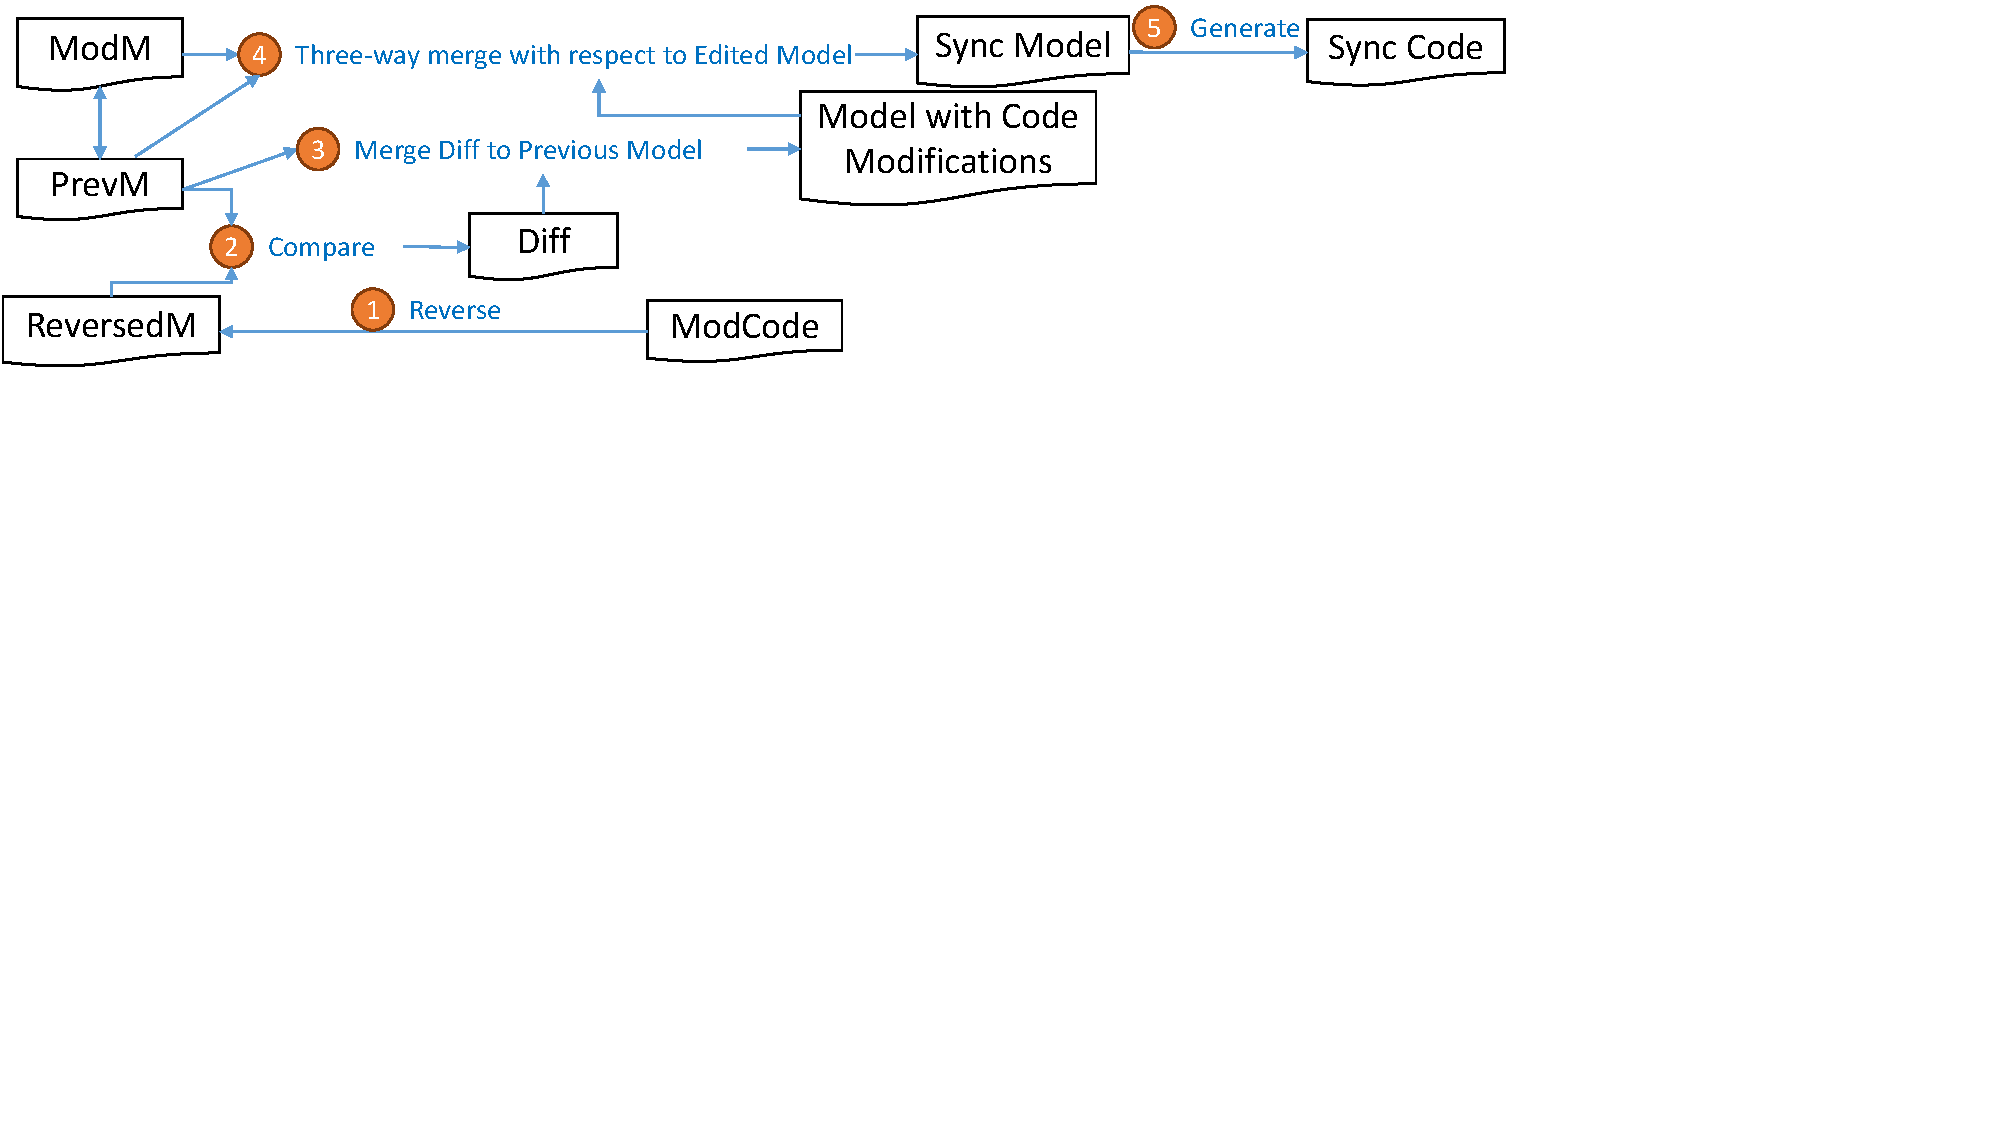
\includegraphics[clip, trim=0cm 12.7cm 7.8cm 0cm, width=\columnwidth]{figures/syncextended.pdf}
	\caption{Synchronization process} 
	\label{fig:syncextended}
\end{figure}

\end{comment}
In our previous work \cite{foster2016}, a model-code synchronization mechanism in case of concurrent modifications is proposed.
%This section extends the pattern to maximize automation and minimize user intervention in synchronization of architecture model and intermediate code.
%In order to keep the paper focused, we abstractly present the synchronization as below.
The mechanism especially requires the availability of several use-cases as followings:

\begin{itemize}[\footnotesize]
	\itemsep0em 
	\item \tb{Batch code generation}: generates and overwrites any existing code from model.
	
	\item \tb{Incremental code generation}: updates the code by propagating changes from the model to the code.
	
	\item \tb{Batch reverse engineering}: creates and overwrites any existing model from code.
	
	\item \tb{Incremental reverse engineering}: updates the model by propagating changes from the code to the model.
\end{itemize}


The batch code generation and reverse engineering are straightforwardly supported by using the proposed bidirectional mapping between the architecture model and code. 
The incremental code generation (ICG) and incremental reverse engineering (IRE) needs a classification and management of modifications made in the model and code.

%\vskip 0.2cm
\noindent
\tb{Incremental code generation:}
Table \ref{table:modelchangeclassification} shows our management of actions for propagating modifications in model to code.
%The modifications can be detected by a model listener.
We make a distinction between structural and behavioral modifications, which result in creating/removing/regenerating the corresponding code part.
Although only add/remove/update are detected, the moving of a model element can be detected as a combination of a removal followed by an addition.  
%Some particular modifications requires the corresponding actions to respect and preserve the user code.
%For example, if the \ttt{sendDataToFifo} method in Listing \ref{lst:producerinteraction} is renamed to \ttt{sendDataFromProducerToFifo} at the model level, the corresponding action consists of several steps: (1) identify the method, at the code level, associated with the operation, at the model level, using the old name \ttt{sendDataToFifo}, which is recorded by the model listener;
%(2) rename the method to \ttt{sendDataFromProducerToFifo} while keeping its parameters and body intact. 



\begin{comment}
\vskip 0.2cm
\noindent
\tb{Code modification classification and management:}
Modifications types in code are similar to that of model consisting of structural and behavioral modifications.
However, we do not support the removal of classes in code because this kind of modification causes conflicts and syntax errors, which require the code to be manually re-factored for reconciliation. 
We believe that an automatic mechanism brought by the regeneration of code caused by the removal can better handle the refactoring.
If the FIFO class is removed in the code, for example, the \ttt{fifo} in \ttt{System} in Listing \ref{lst:architectureprescribed} must be retyped or removed.
If not, a compilation error is raised.
% Please add the following required packages to your document preamble:
% \usepackage{multirow}
\end{comment}
\begin{table*}[]
	\scriptsize
	\centering
	\caption{Model change classification and management}
	\label{table:modelchangeclassification}
	\begin{tabular}{|l|p{3cm}|l|p{9.5cm}|}
		\hline
		\multicolumn{2}{|c|}{Element type}                              & \multicolumn{1}{c|}{Modification type} & \multicolumn{1}{c|}{Action}                                                                              \\ \hline
		\multirow{3}{*}{Structure} & Part/Port/Connector                & Add/Remove/Update                      & Regenerate and re-transform code for the component containing the modified model element.                                                           \\ \cline{2-4} 
		& Class/Component/Interface          & Add/Remove/Update                      & Create/Remove/Update the corresponding code file(s). If the modification is remove or rename (update), regenerate the classes/components/interfaces that depend on the removed/renamed element. 
		For example, regenerate the classes containing attributes typed by the deleted types to avoid unknown type problems during compilation.                                                              \\ \cline{2-4} 
		& Property                           & Add/Remove/Update                      & Regenerate the corresponding class                                               \\ \hline
		Behavior  & Operation                          & Add/Remove/Update                      & Regenerate the corresponding class                           \\ \cline{2-4} 
		& UML State Machine & Add/Remove/Update                                 & Regenerate and transform code for the component containing the state machine                                           \\ \hline
	\end{tabular}
\end{table*}

%Using these use-cases and the bidirectional traceability facilitated by XSeparation during code generation, the concurrent modifications in model and code can be synchronized by our previous methodological pattern.

%\vspace{0.1cm}
\noindent
\tb{Incremental reverse engineering:}
Our IRE, with specificity in text, is similar to change-driven transformation (CDT) \cite{rath2009change}.
The latter listens to changes made in a model and uses predefined rules to propagate the changes back to another model.
However, CDT cannot be applied directly to propagate changes in code back to model because detection of changes in code is non-trivial.
The approach in \cite{kramer2015change} records every developer operation by creating a specific code editor.
However, this approach is not reliable because it is hard to monitor all of developer modifications if the developer uses different editors to modify the code.

In our approach, we do not record all of modifications made to code elements.
We use a \ti{File Tracker} to detect which files are changed by developers.
This kind of tracking is much easier to realize and more realistic than the above approaches. 
It is also supported by several tools such as Git.
The details of our approach are shown in Fig. \ref{fig:incrementalreverse}.

The file tracker monitors all of the code files generated from the architecture model.
The tracker does not listen to specific changes to programming language elements such as renaming an attribute or adding a method.
After all of modifications made in the code, the tracker returns a list of files which were changed during modification.
We do not allow renaming or deleting a class because doing these modifications at the code level requires doing some additional re-factorings.
For example, deleting a class requires re-typing class attributes typed by this deleted class.  
We believe that working at the model level is more suitable to these modifications because the re-factorings can be done through code re-generation from the modified model.
Furthermore, the IRE then needs to propagate modifications in the code within the class scope (attributes, methods, state machines) back to the model. 
 
The modified files and the model are then used as input for reverse engineering.
For each modified file, the IRE for each code element in the file follows a \tb{Update-Create-Delete} strategy as followings: 

\begin{itemize}
	\item Update: Finding a model element matching with the code element by using the name and type of the code element to look for the corresponding model element. 
	If exists, using the information of the code element to update the model element.
	For example, if we modify the \ti{entryCheck} method body in Fig. \ref{fig:approachexample} \encircle{d}, the IRE will automatically propagate the changed body to the architecture model as a block of text.
	
	\item Create: If do not find a matching model element, creating a model element corresponding to the code element. 
	For example, if a programmer adds a state to the state machine example in Fig. \ref{fig:approachexample} \encircle{d}, a UML state will be created in the model.
	
	\item Delete: UML elements (attributes, ports, connectors, methods, state machines, and events), which are not touched during the IRE, are deleted because these elements are implicitly removed by programmers during code modification.
\end{itemize}

It is worth noting that a renaming in code will be considered as an addition followed by a deletion at the model level.

%We do not allow to rename/delete a class at the code level.

\begin{figure}
	\centering
	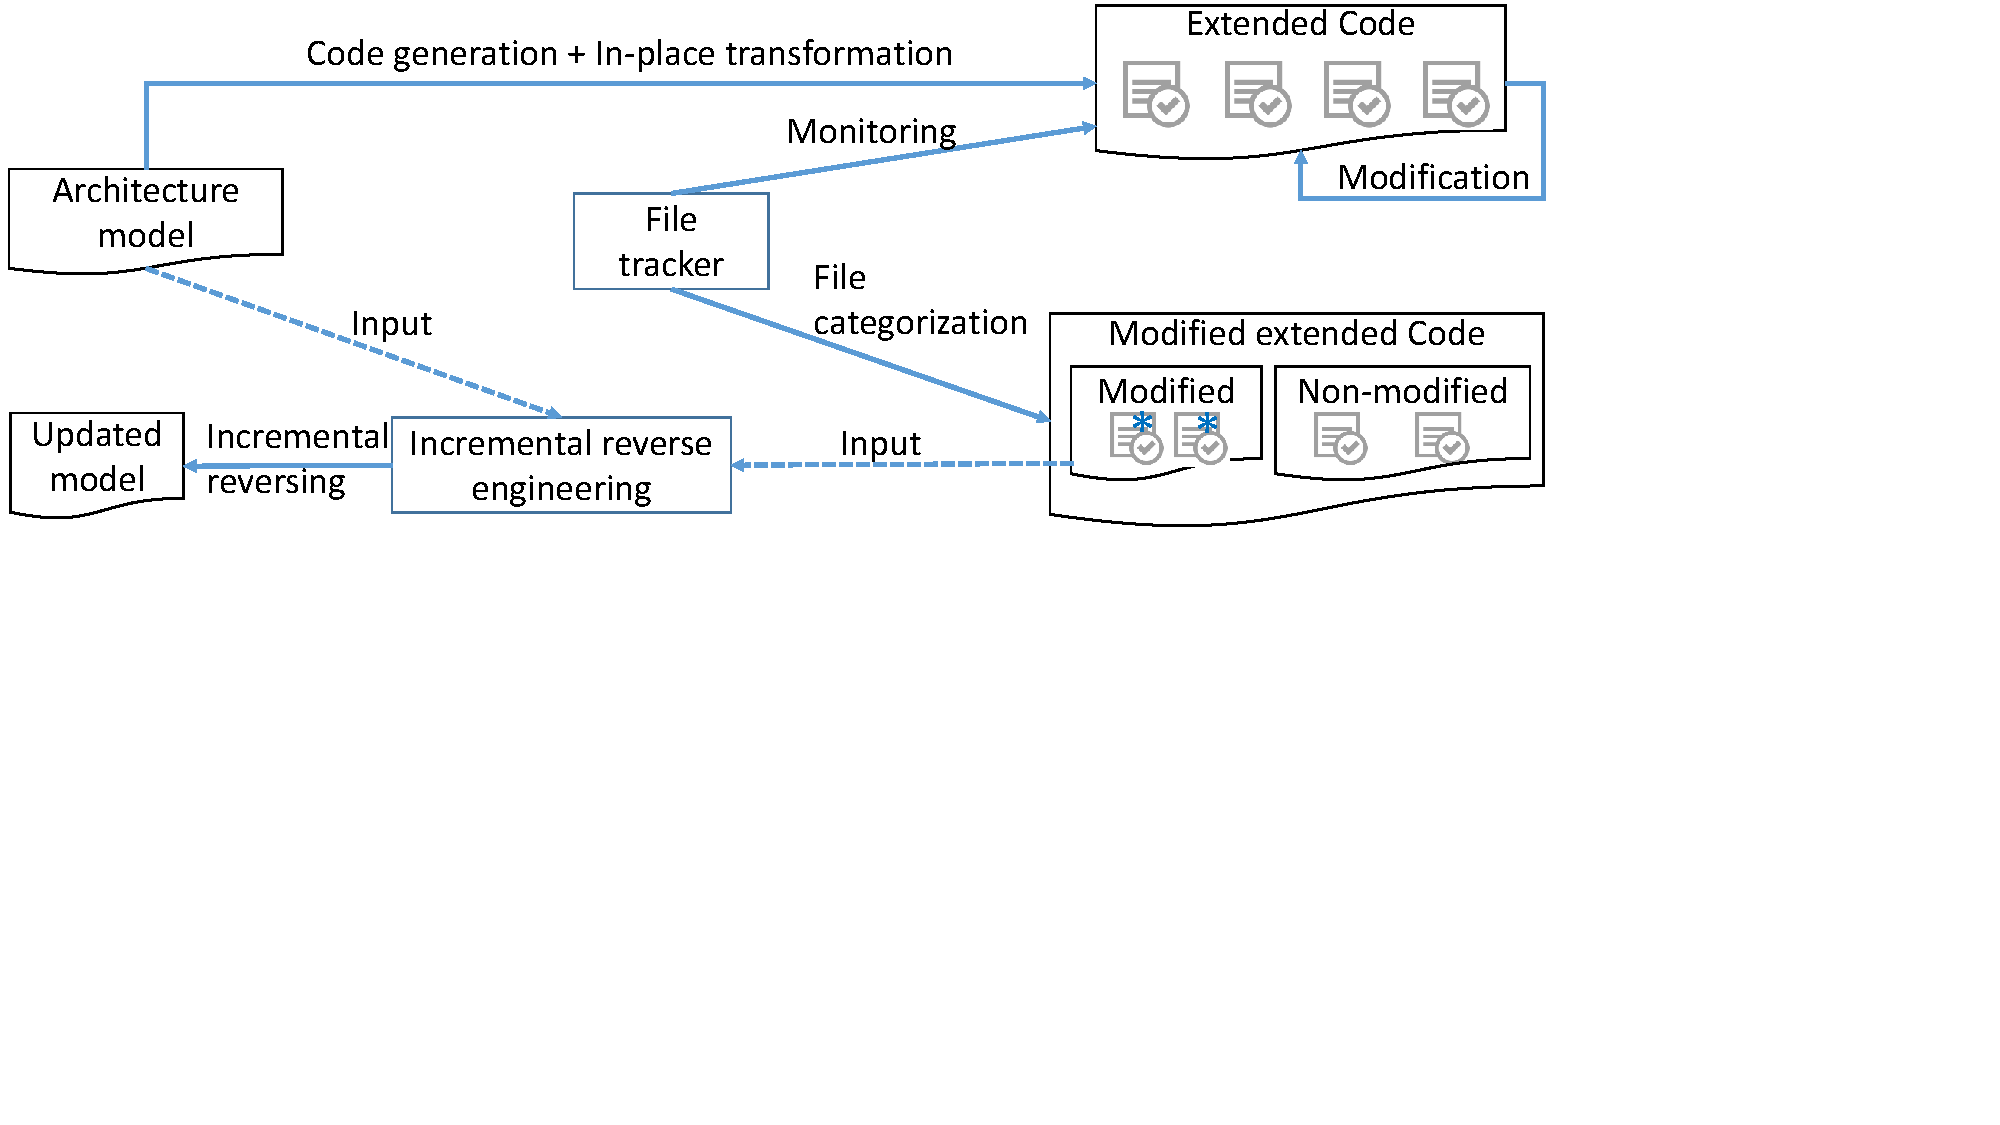
\includegraphics[clip, trim=0cm 10.1cm 7.0cm 0cm, width=0.9\columnwidth]{figures/incrementalreverse.pdf}
	\caption{Incremental reverse engineering with file tracker} 
	\label{fig:incrementalreverse}
\end{figure}

In the next section, we describe our experiments to evaluate our approach.


%\begin{comment}
\begin{table}[]
	\centering
	\caption{My caption}
	\label{my-label}
	\begin{tabular}{lllll}
		UML                  & XGC                      &  & OO                             & C++                 \\ \cline{1-2} \cline{4-5} 
		Class component      & Class                    &  & Class                          & Class               \\ \cline{1-2} \cline{4-5} 
		Part                 & Part                     &  & Composition attribute          & Attribute           \\ \cline{1-2} \cline{4-5} 
		Port  (data/control) & Port                     &  & Attribute                      & Reference Attribute \\ \cline{1-2} \cline{4-5} 
		Many ports           & Multiple-port            &  & Multiple interface realization & --                  \\ \cline{1-2} \cline{4-5} 
		Connector            & Binding (static+dynamic) &  & --                             & Methods             \\ \cline{1-2} \cline{4-5} 
		Interface            & Class/Interface          &  & Interface                      & Class               \\ \cline{1-2} \cline{4-5} 
		Signal               & Class                    &  & Class                          & Class/Struct        \\ \cline{1-2} \cline{4-5} 
		State machine        & state\_machine           &  & --                             & --                  \\ \cline{1-2} \cline{4-5} 
		State                & state                    &  & --                             & --                  \\ \cline{1-2} \cline{4-5} 
		Region               & region                   &  & --                             & --                  \\ \cline{1-2} \cline{4-5} 
		CallEvent            & call\_event              &  & --                             & --                  \\ \cline{1-2} \cline{4-5} 
		TimeEvent            & time\_event              &  & --                             & --                  \\ \cline{1-2} \cline{4-5} 
		ChangeEvent          & change\_event            &  & --                             & --                  \\ \cline{1-2} \cline{4-5} 
		SignalEvent          & signal\_event            &  & --                             & --                  \\ \cline{1-2} \cline{4-5} 
		Any                  & any                      &  & --                             & --                  \\ \cline{1-2} \cline{4-5} 
		Pseudo state         & pseudo\_state            &  & --                             & --                  \\ \cline{1-2} \cline{4-5} 
		Action/Effect        & Method                   &  & Method                         & Method             
	\end{tabular}
\end{table}
\end{comment}

\begin{table}[]
	\centering
	\caption{Mapping between UML and Examples of Extended Language}
	\label{table:mapping}
	\begin{tabular}{lll}
		UML                                                                      & Extended Language                                                                                & Code example in Fig. \ref{fig:approachexample}                                                                               \\ \hline
		\begin{tabular}[c]{@{}l@{}}Port requiring \\ an interface \ti{I}\end{tabular} & \begin{tabular}[c]{@{}l@{}}Attribute typed \\ by \ti{RequiredPort}\textless I\textgreater\end{tabular} & \begin{tabular}[c]{@{}l@{}}Ports \ti{pPush} and \ti{pPull} at lines\\ 21 and 25\end{tabular}         \\ \hline
		\begin{tabular}[c]{@{}l@{}}Port providing \\ an interface \ti{I}\end{tabular} & \begin{tabular}[c]{@{}l@{}}Attribute typed\\ by \ti{ProvidedPort}\textless I\textgreater\end{tabular}  & \begin{tabular}[c]{@{}l@{}}Ports \ti{pPush} and \ti{pPull} at \\ lines 29-30\end{tabular}            \\ \hline
		Connector                                                                & Binding                                                                                        & Lines 7-8                                                                                  \\ \hline
		State Machine                                                            & \ti{StateMachine}                                                                                     & \begin{tabular}[c]{@{}l@{}}The FIFO state machine at \\ lines 34-59\end{tabular}           \\ \hline
		State                                                                    & \ti{State/InitialState}                                                                               & \begin{tabular}[c]{@{}l@{}}State \ti{SignalChecking} at \\ lines 36-39\end{tabular}             \\ \hline
		Region                                                                   & \ti{Region}                                                                                           & Not shown in this paper                                                                                 \\ \hline
		Pseudo state                                                             & \begin{tabular}[c]{@{}l@{}}Attribute typed \\ by pseudo type\end{tabular}                        & \begin{tabular}[c]{@{}l@{}}The \ti{dataChoice} pseudo state \\ at line 49\end{tabular}          \\ \hline
		Action/Effect                                                            & Method                                                                                           & Methods at lines 60-65       \\ \hline
		Transitions                                                           & Transition table                                                                                           & Transition table at lines 51-58	\\ \hline
		Event                                                            & Event                                                                                           & The call event at line 50                                                             
	\end{tabular}
\end{table}



%
This section describes RAOES's process to synchronize a model with UML component, UML class, UML State Machine concepts and front-end code in case that these artifacts concurrently evolve.
We assume then use of an integrated development environment (IDE) %used by software architects and programmers 
offering the use-cases defined in Section \ref{subsec:mdrtebackground}. 
%Although, the pattern is presented in a model-code synchronization-oriented way, it is flexibly extensible to any artifacts. 
%For the sake of generality, we postulate that the architect and programmer are actors with starkly opposite development practices.
The process allows concurrent modifications made to the model
and front-end code so that in the end we obtain a full system.
%rather than just architectural design for the former,
%and code implementation for the latter.

Before going to the synchronization detail, we give the summary of the mapping from UML to XSeparation-generated code concepts as in Table \ref{table:mapping}.
The majority of the mapping elements are one-to-one, which facilitate the synchronization.


We propose two synchronization strategies.
The rationale behind our strategies
is to represent one artifact (model or front-end code) in the language of its corresponding other artifact (front-end code or model).
%These two can then be compared. 
For this, we define the
concept of a \ttt{synchronization artifact}:

\begin{definition}[Synchronization artifact]
	An artifact used to synchronize a model and its corresponding front-end code
	is called a synchronization artifact.
	It is an image of one of the artifacts, either the model or the front-end code.
	In this context, an image $I$ of an artifact $A$ is a copy of $A$ obtained by
	transforming $A$ to $I$. $A$ and $I$ are semantically equivalent but are specified in different languages.
\end{definition}

For example, a synchronization artifact (SA) can be code that was generated from the edited model in batch mode.
In that case, it is code that represents an image of the edited model (being image requires that the model is able to be reconstructed from the code).

Using the concept of SA, two strategies are
proposed: one in which the SA is code,
and the other in which the SA is a model.
The developer can choose to either use these two use-cases of the IDE. 
The choice may be determined by
preferred development practices or the availability of suitable tools (e.g. the programmer
may prefer to synchronize two artifacts, both represented
in the same programming language, since he prefers to
work exclusively with code).

Figure \ref{fig:scenario3} shows the first synchronization
strategy based on using front-end code as SA.
The general steps of the process shown in Figure \ref{fig:scenario3} are described as follows:

\begin{figure}
	\centering
	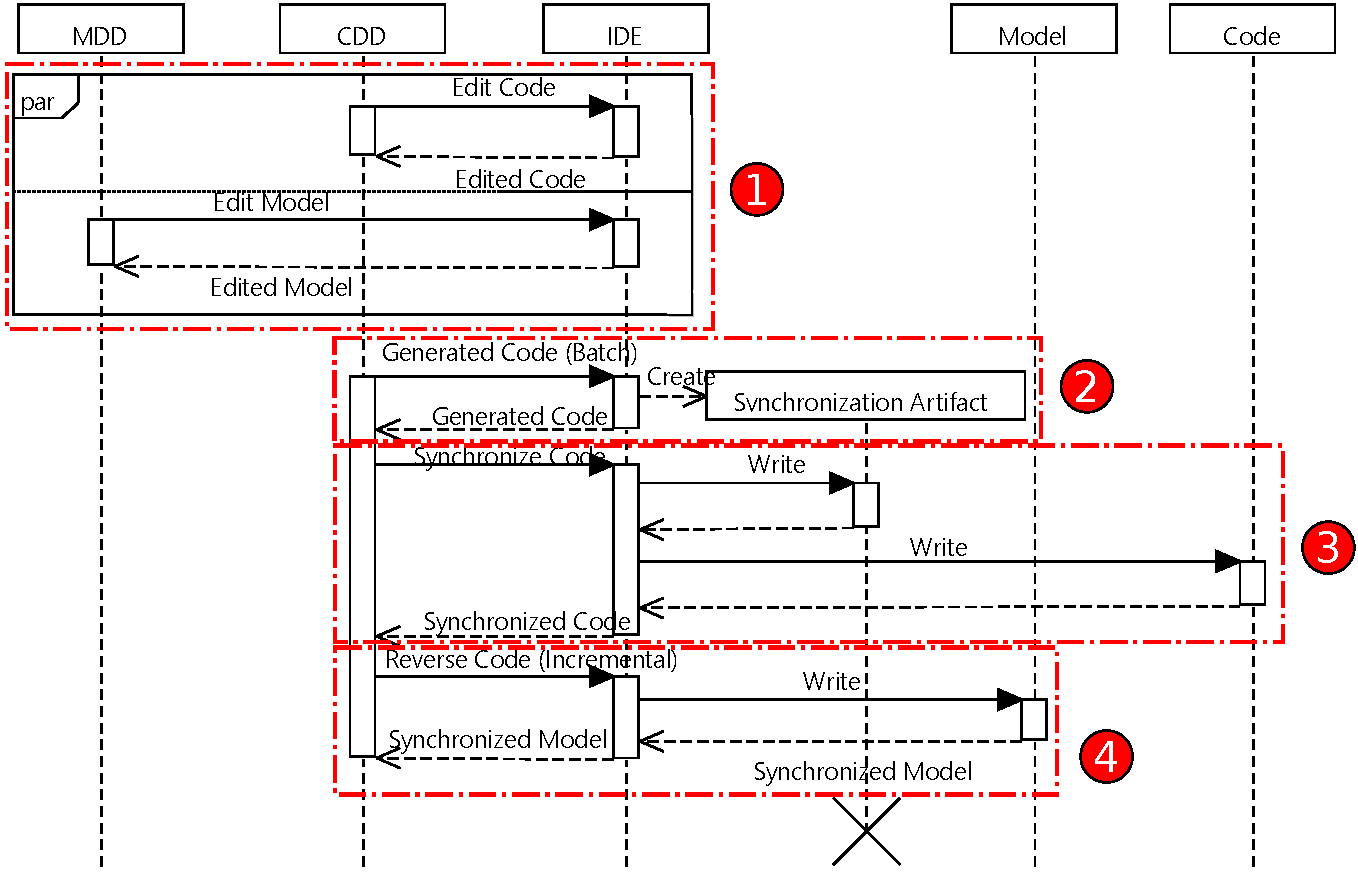
\includegraphics[width = \columnwidth]{figures/scenario3_seq}
	\caption{Synchronization process, in which the model and the code are concurrently edited with code as the SA (CDD = Code-Driven Developer = Programmer, MDD = Model-Driven Developer = Software Architect, Code = C++ front-end code). The API calls for Model and Code are represented generically as "Read" and "Write".}
	\label{fig:scenario3}
\end{figure}

\begin{description}[\footnotesize]
	\item[Step 1] Both the model and code may be edited concurrently.
	%(To simplify Figure \ref{fig:scenario3}, we don't show the Read and Write interactions for this step.)
	%After both artifacts have been edited concurrently, we need to synchronize them.	
	\item[Step 2] First we create an SA from the edited model by generating front-end code in batch mode.
	This SA is code and it is an image of the edited model.	
	
	\item[Step 3] The SA is synchronized with the edited code. Since the SA
	is code itself, this step is done with the \texttt{Synchronize Code} use-case of the IDE.
	
	\item[Step 4] Once SA and edited code are synchronized, the former is reversed incrementally to update the edited model.
\end{description}

The second strategy, based on using the model as the SA,
is the opposite of the first strategy. 
In the second strategy, the SA is
obtained by reversing the edited code in batch mode.
Afterwards the SA is synchronized with the edited model.
Finally, we generate code incrementally from the SA to update the edited code.

%Figure \ref{fig:strategy2} shows the synchronization strategy based on using model as the synchronization artifact.
%This strategy is the opposite of the strategy presented in Figure \ref{fig:strategy1}. Its steps are described as follows:
%
%\begin{center}
%\textbf{\textit{- Steps of synchronization strategy 2 -}}
%\end{center}
%\begin{description}
%	\item[Step 1] The synchronization artifact is obtained by reversing the edited code in batch mode.
%	\item[Step 2] Afterwards the synchronization artifact is synchronized with the edited model.
%	\item[Step 3] Finally, we generate code incrementally from the synchronization artifact to update the edited code.
%\end{description}
%
%\begin{figure}
%\centering
%\includegraphics[width=\columnwidth]{figures/strategy2}
%\caption{Synchronization strategy 2 using model as synchronization artifact}
%\label{fig:strategy2}
%\end{figure}

The actors may even use both strategies, successively, as a kind of hybrid strategy.
This may be useful
when developers want to synchronize some parts of the system using one strategy,
and other parts using the other strategy. %For example, they may choose
%to synchronize method bodies using strategy 1, where the synchronization artifact is code.
%Then strategy 2, in which the synchronization artifact is a model, is used to
%to synchronize architectural elements of the system.

%In reality of collaboration, there are of course conflicts between editions made by developers to their respective baseline artifact.
%Two approaches are proposed to reconcile these conflicts.
%In the first approach, we let the developers explicitly determine which edition should be kept in the synchronization process.
%This is based on the \texttt{Compare and Merge} paradigm proposed by model/code merge tools such as \textbf{EMF Compare} or \textbf{Git}.  
%The second approach extends the semi-automated conflict resolution presented in \cite{Hermann2012}.
%Specifically, our approach records editions made to artifacts (see Section \ref{sec:implementation} for more information about edition listening), decides whether editions are \textit{conflict-free} or not, and automatically bi-directionally merges or interactively shows the developers in-conflict editions.
%For example, if an MDD adds an attribute to a class by using graphical modeling tools and a CDD renames the class.
%Two editions are detected and asserted as conflict-free. The automated merge therefore is used for reconciliation. 

%In the next section we propose an implementation
%of an IDE and the proposed synchronization processes.

%\subsection{Illustration example}
